\documentclass[12pt,openright,a4paper]{article}

\usepackage{hyperref}
\usepackage[T1]{fontenc}
\usepackage[utf8]{inputenc}
\usepackage[italian]{babel}
\usepackage{amsmath}
\usepackage{amssymb}
\usepackage{caption}
\usepackage{graphicx, floatflt}
\usepackage{booktabs}
\usepackage{textcomp}
\usepackage{subfig}

% permette di inserire le note a margine
\usepackage{marginnote}


\begin{document}
\title{Classificazione di Soggetti ADNI-2 Tramite Analisi Di Matrici di Correlazione}
\author{Carlo Mengucci}

\maketitle

\tableofcontents

\section{Struttura e Utilizzo del Database}

Dei 403 soggetti totali sono stati utilizzati 232 soggetti a seguito di operazioni di filtraggio e dell'individuazione di discrepanze nelle procedure di normalizzazione. 

E' infatti possibile riscontrare la presenza di due gruppi distinti all'interno del database, dei quali è stato preso in considerazione il più numeroso, formato da circa 300 soggetti.

Dei 300 soggetti, 232 sono stati utilizzati per l'elaborazione finale. Sono infatti stati esclusi dal \textit{training} i soggetti appartenenti alla categoria \textit{MCI, Mild Cognitive Impairment}, in modo da considerare esclusivamente soggetti \textit{san}i \textit{NC} e \textit{malati} \textit{AD}; è stata in questo modo eliminata dall'analisi la componente di conversione. 

 La presenza di soggetti per il gruppo \textit{AD} è del $63 \% $ mentre il restante  $37 \%$ dei 232 soggetti considerati appartiene al gruppo \textit{NC}.

Ad ogni soggetto è associata una matrice di correlazione $N\times N$, $N=549$, Ognuno degli N elementi rappresenta un \textit{Macrovoxel} di cui è estratta la correlazione \textit{topologica} rispetto a tutte le altre componenti del sistema. Ogni \textit{Macrovoxel} è definito su un insieme di $3\cdot10^3$ Voxel.

\section{Separazione tramite Wishart Likelihood Test}

Le matrici di correlazione sono per definizione simmetriche definite positive; seguono dunque in maniera naturale la distribuzione di Wishart.

Il numero $n$ di gradi di libertà del sistema è dato dal campionamento $(n=3\cdot 10^3)$ del singolo Macrovoxel.

Utilizzando come matrice di scala la matrice data dalla media delle matrici di correlazione delle due categorie di soggetti, è possibile stimare la Wishart attesa per le categorie stesse.

Un approccio di questo tipo permette la classificazione di ogni soggetto in base alla propria distanza dalle distribuzioni rappresentative delle categorie, in termini di \textit{LogPDF}, come definito dalla eq.(\ref{pdf-score}):

\begin{equation}
score_{subj }= logP_{W}(\Sigma_{subj}\mid n, \hat{\Sigma}_{AD})-logP_{W}(\Sigma_{subj}\mid n,\hat{\Sigma}_{NC})
\label{pdf-score}
\end{equation}

dove $\Sigma_{subj}$ rappresenta la matrice del singolo soggetto e $\hat{\Sigma}_{AD,NC}$ è la matrice media di categoria.

Sostanzialmente è utilizzato un \textit{Likelihood Ratio Test} per stabilire l'appartenenza del singolo soggetto alla categoria dei sani o dei malati.

\subsection{Single Feature Likelihood Ratio}

L'algoritmo implementato permette un ulteriore livello di analisi.

Per ogni paziente viene infatti calcolato un vettore contenente gli \textit{score} relativi alle singole features; ossia alle 549 componenti del sistema.

Per ogni elemento della matrice di correlazione, viene calcolata la matrice ridotta che permette di stabilire la variazione di \textit{Likelihood Ratio Score} per il soggetto se la componente in questione non fosse stata osservata; in questo modo è possibile stabilire quali \textit{features} hanno un peso maggiore nell'attribuzione dell'appartenenza all'una o all'altra categoria.

Il risultato dell'elaborazione è dunque una mappa contenente un vettore per ogni singolo paziente, al cui interno sono contenuti gli \textit{scores} relativi alle singole features.

\subsection{Pipeline}

\begin{figure}[!h]
\centering
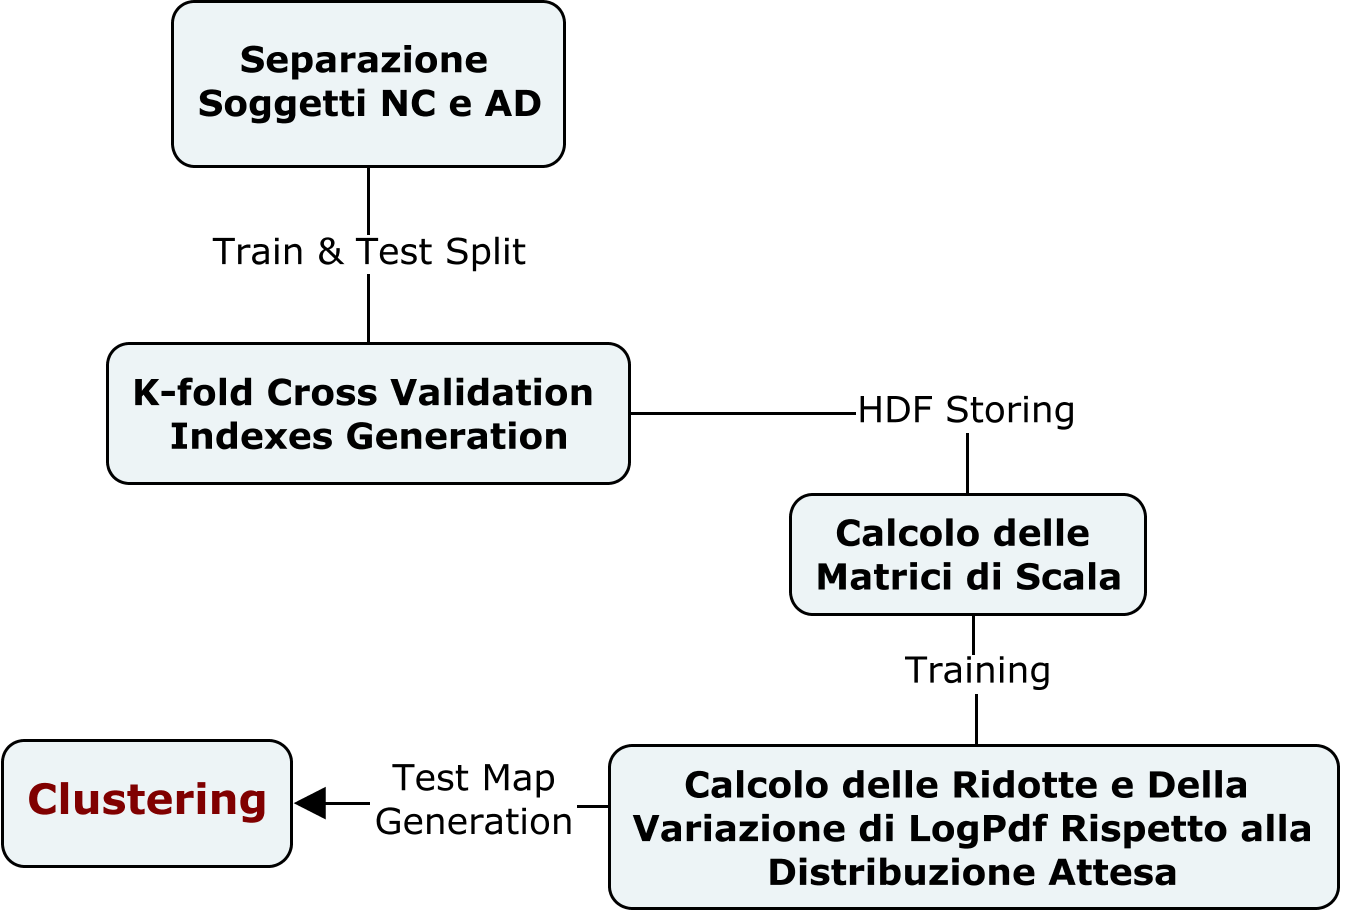
\includegraphics[scale=0.18]{ADNI-alg}
\caption{\textit{Schema di Workflow della pipeline di elaborazione}}
\label{ADNI-alg}
\end{figure}

In figura (\ref{ADNI-alg}) è riportato lo schema di funzionamento dell'intera pipeline. Viene testata la capacità di discriminare tra \textit{NC} e \textit{AD} attraverso un processo di \textit{supervised learning}.

A seguito di una divisione iniziale nelle due classi, vengono separati i soggetti in \textit{train} e \textit{test} secondo il classico split $90 \%- 10 \%$ per ogni batch della \textit{K-fold cross-validation}.

Da ogni batch di training è calcolata la matrice di scala da cui è generata la distribuzione che viene confrontata con il corrispettivo batch di test.

Per ogni soggetto dei batch di test è infine generato un vettore contenente gli \textit{scores} relativi alle singole features, i quali vanno a comporre le mappe finali su cui viene effettuata la classificazione.

\subsection{Risultati}

Per la classificazione finale, effetuata sulle mappe \textit{soggetto-vettore degli scores},  è stata utilizzata una SVM a \textit{Kernel Lineare} e parametro $C=1$. Gli scores di classificazione, in questo caso \textit{l'accuracy},  sono quindi stimati tramite una cross-validazione 10-fold stratificata. 

Il risultato è un'\textit{accuracy} del  $100\%$. Questo risultato è confermato anche dai picchi in fig.(\ref{logpdf-dist}), ottenuti riducendo il vettore di score ad un singolo scalare per ogni paziente tramite  somma.

Si può notare come utilizzando questo semplice procedimento la discriminazione ottenuta è ottima.

\begin{figure}[!h]
\centering
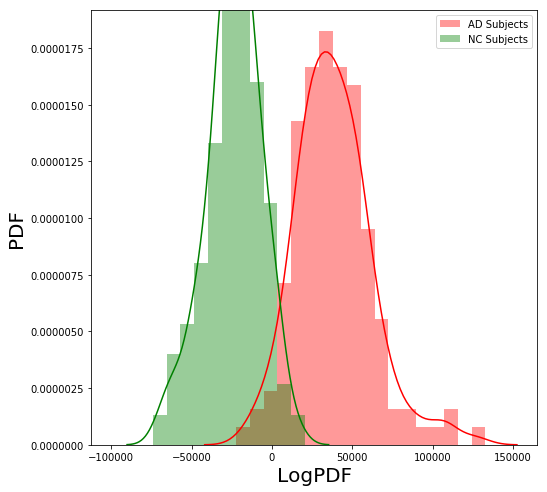
\includegraphics[scale=0.6]{logpdf-dist}
\caption{\textit{Distribuzioni della somma degli scores per paziente. Le classi sono ben distinte anche riducendo ad un unico score l'informazione sui soggetti.}}
\label{logpdf-dist}
\end{figure}


\end{document}

